% !TeX document-id = {9ccc6fb7-c5f4-4308-9c17-4c226ad62230}
%%%%%%
%
% $Autor: Alpizar, Kumari, JK $
% $Datum: 2023-01-31 11:59:00Z $
% $Version: 1.0.0 $
%
%
% !TeX encoding = utf8
% !TeX root = Rename
% !TeX TXS-program:bibliography = txs:///biber
%
%%%%%%

\chapter{Appendix}

In this section it is included additional information, relevant for the project development among other technical, financial and theoretical explanations related to the Digitization of Meter's Digits, with an ESP32-CAM.
  
\bigskip

%%%%%%%%%%%%%%%%%%%%%%%%%%%%%%%
\section{Material List}
\ac{hw} List of materials required for the project:
\begin{itemize}
	\item \textbf{ESP32-CAM AI-Thinker} \\
	\begin{itemize}
		\item Description: ESP32-CAM is a low-cost ESP32-based development board with onboard camera (OV2640), small in size. It is an ideal solution for \ac{iot} application, prototypes constructions and \ac{diy} projects. The board integrates WiFi, traditional Bluetooth and low power BLE , with 2 high-performance 32-bit LX6 CPUs.
		\item Link Datasheet: \url{https://media.digikey.com/pdf/Data%20Sheets/DFRobot%20PDFs/DFR0602_Web.pdf}
		\item Cost: Approximately 10 Euro.
	\end{itemize}
	\begin{figure}  [H]
		\begin{center}
			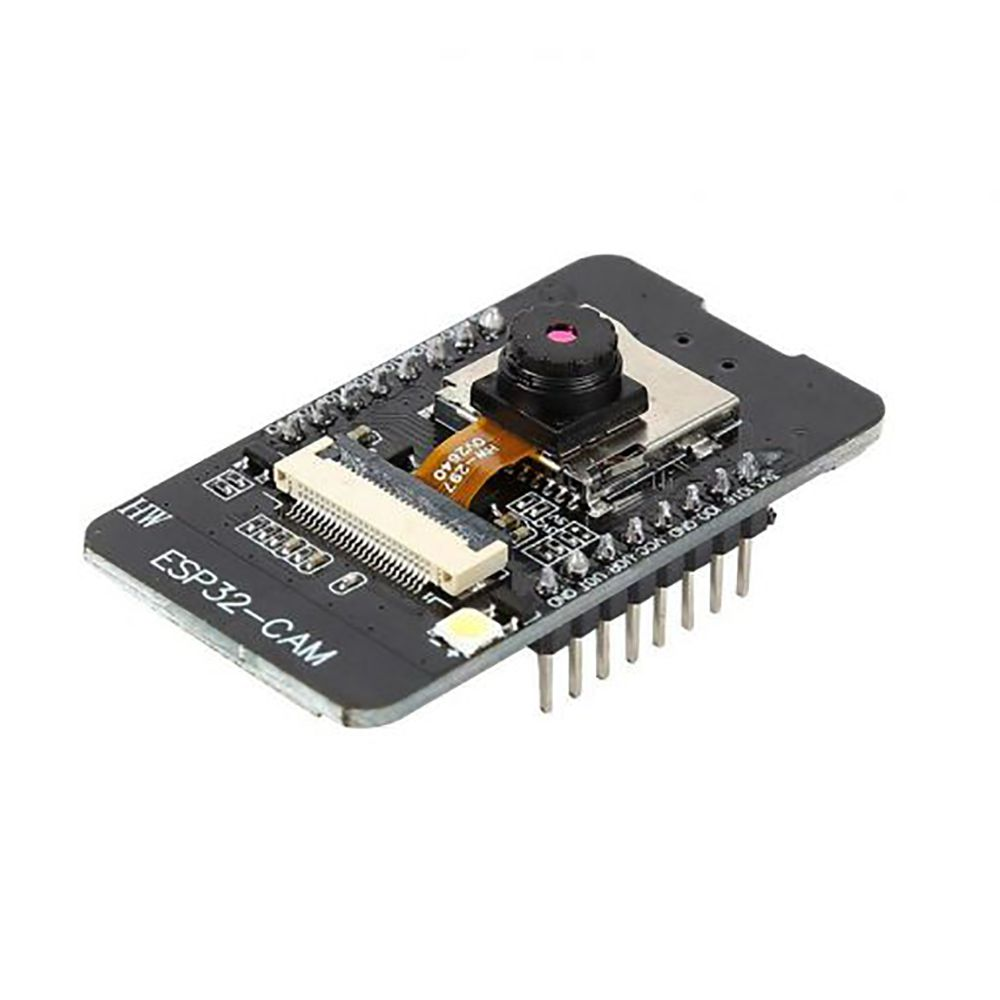
\includegraphics[width=12cm, height=6cm]{ListMaterialESP32CAM}
			\caption{ESP32-CAM.} 
			\label{fig:ESP32-CAM.}
			\footnotesize \textbf{Reference:} \autocite{Elektor:2022}
		\end{center}
	\end{figure}	

	\item\textbf{OV2640 Camera} \\
	\begin{itemize}
			\item Description: OV2640 Camera is a 2 Megapixel OV2640 camera module with an f3. 6mm lens. It contains a 24pin FPC interface. A wide-angle lens and 1632 x 1232 high resolution make it a perfect camera for Grove AI HAT for Edge Computing and other Sipeed serial board.
			\item Link Datasheet: \url{https://www.uctronics.com/download/cam_module/OV2640DS.pdf}
			\item Cost: Approximately 5 Euro.
	\end{itemize}
	\begin{figure}  [H]
		\begin{center}
			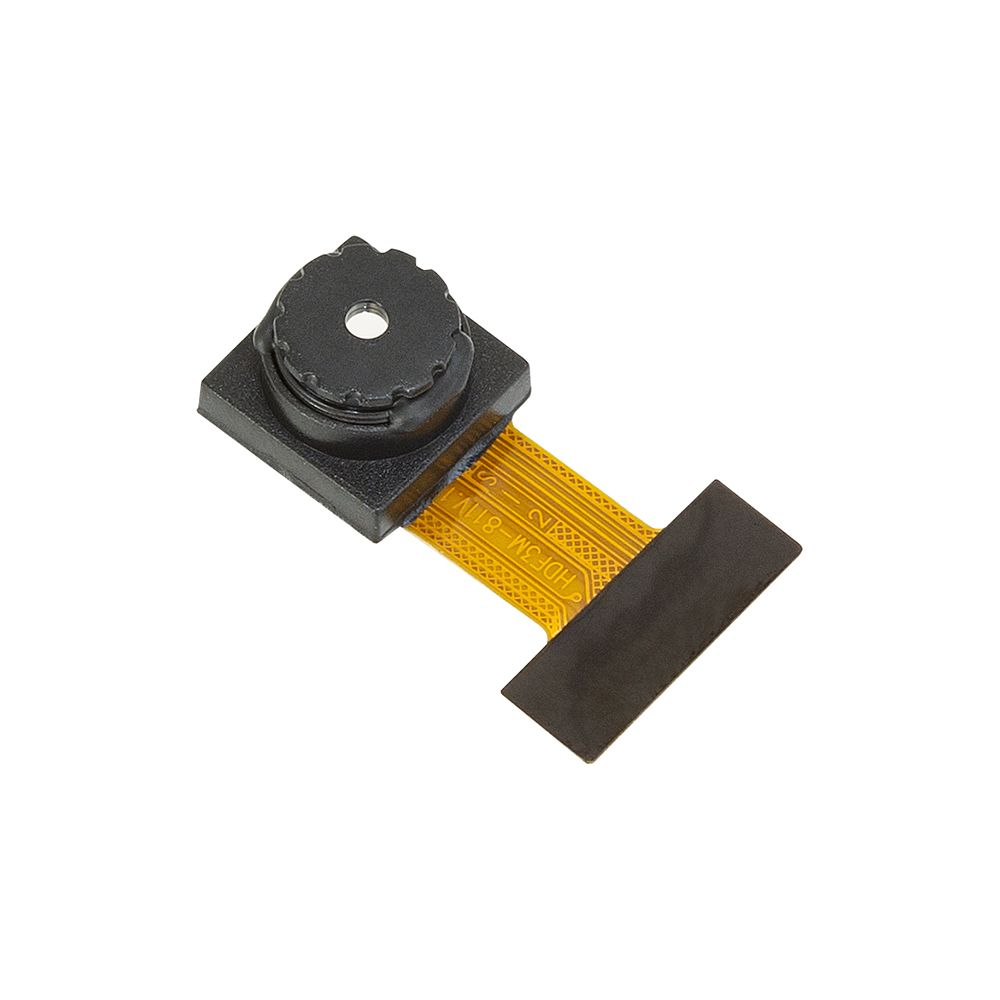
\includegraphics[width=12cm, height=6cm]{OV2640}
			\caption{OV2640 Camera.} 
			\label{fig:OV2640 Camera.}
			\footnotesize \textbf{Reference:} \autocite{ArduCam:2022}
		\end{center}
	\end{figure}	
	
	\item \textbf{ESP32-CAM-MB USB Programmer} \\
	\begin{itemize}
		\item Description: The ESP32-CAM AI-Thinker MB programmer is a shield that can be attached to the ESP32-CAM board GPIOs. The programmer comes with the CH340C USB to serial chip; this allows serial communication to the ESP32-CAM using the USB port on the shield. Additionally, the shield also comes with a RESET and a BOOT (IO0) buttons. This may be useful to easily reset the ESP32-CAM or put it into flashing mode.
		\item Link Datasheet: N/A
		\item Cost: Approximately 2 Euro.
	\end{itemize}
	\begin{figure}  [H]
		\begin{center}
			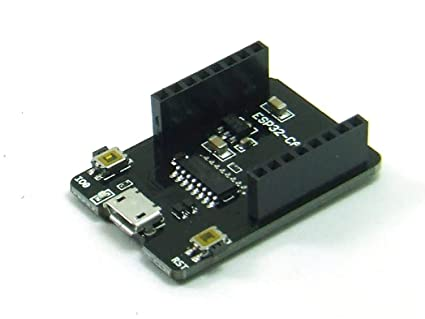
\includegraphics[width=12cm, height=6cm]{ListMaterialESP32MB}
			\caption{ESP32-CAM-MB USB Programmer.} 
			\label{fig:ESP32-CAM-MB USB Programmer.}
			\footnotesize \textbf{Reference:} \autocite{Amazon:2022}
		\end{center}
	\end{figure}	

	\item \textbf{Secure Digital (SD) Card \(16 GB\)} \\
	\begin{itemize}
		\item Description: A memory Secure Digital card is an electronic data storage device used for storing digital information, typically using flash memory. These are commonly used in digital portable electronic devices. They allow adding memory to such devices using a card in a socket instead of a protruding USB flash drives.
		\item Link Datasheet: \url{https://www.intenso.de/en/products/memory-cards/microsd-card-class-10}
		\item Cost: Approximately 5 Euro.
	\end{itemize}
	\begin{figure}  [H]
		\begin{center}
			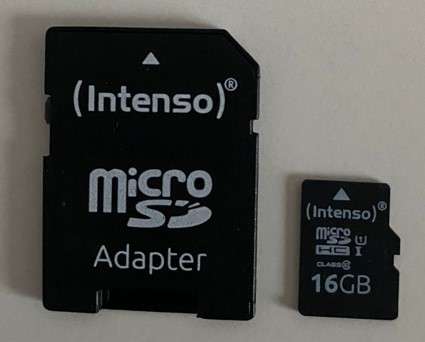
\includegraphics[width=12cm, height=6cm]{ListMaterialSDCard}
			\caption{Secure Digital Card.} 
			\label{fig:Secure Digital Card.}
		\end{center}
	\end{figure}	

	\item \textbf{ESP32-CAM Case} \\
	\begin{itemize}
		\item Description: A case to store the ESP32-CAM module to make it easy for the user transportation, install, and handle.
	\end{itemize}
\begin{figure}  [H]
	\begin{center}
		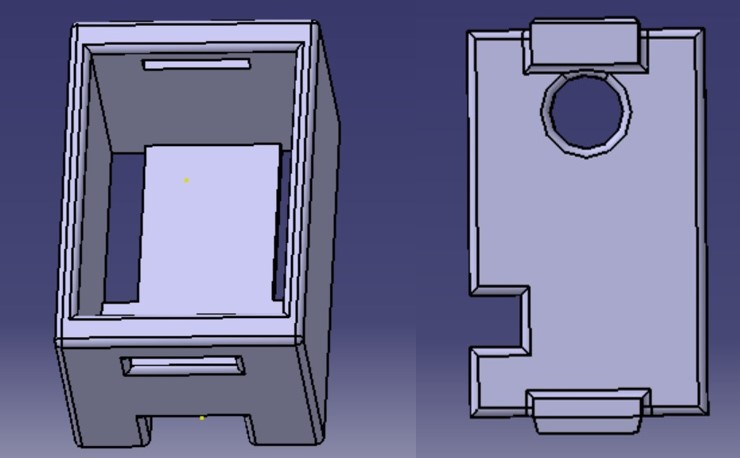
\includegraphics[width=12cm, height=8cm]{CamCase}
		\caption{ESP32-CAM Case.} 
		\label{fig:ESP32-CAM Case.}
		\footnotesize \textbf{Reference:} Designed by Author
	\end{center}
\end{figure}	

	\item \textbf{USB cable - USB A / micro USB B}\\
	\begin{itemize}
		\item Description: USB 2.0 cable with A Male to Micro B connectors is a High-Speed Transmission device that supports up to 480 Mbps. It is mostly used for charging Android phones and tablets or connecting \ac{pc} peripherals such as hard drives, printers, and more. In this specific case, to enable the communication between \ac{pc} and ESP32-CAM.
		\item Link Datasheet: \url{https://www.tme.eu/Document/700e9581ffc48a630c6d37ae87e788bc/esb22.pdf}
		\item Cost: Approximately 3 Euro.
	\end{itemize}
	\begin{figure}  [H]
		\begin{center}
			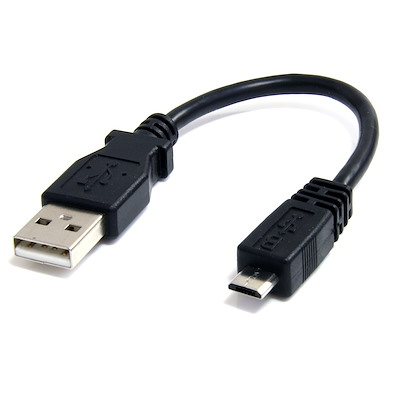
\includegraphics[width=12cm, height=6cm]{ListMaterialUSB}
			\caption{USB cable - USB A / micro USB B.} 
			\label{fig:USB cable - USB A / micro USB B.}
			\footnotesize \textbf{Reference:} \autocite{Tradeinn:2022}
		\end{center}
	\end{figure}	
\end{itemize}
\ac{sw} List of materials required for the project:
\begin{itemize}
	\item \textbf{Python v3.10.} \\
	\begin{itemize}
	\item Description: Python is a computer programming language often used to build websites and software, automate tasks, and conduct data analysis. Python is a general-purpose language, meaning it can be used to create a variety of different programs and isn't specialized for any specific problems.
	\item Link Release Notes: \url{https://docs.python.org/3/whatsnew/3.10.html}
	\item Cost: FREE - Open source.
\end{itemize}
\begin{figure}  [H]
	\begin{center}
		
\includegraphics[width=12cm, height=6cm]{ListMaterialPython}
		\caption{Python 3.10.} 
		\label{fig:Python 3.10.}
	\end{center}
\end{figure}			
		
	\item \textbf{Visual Studio Code v1.73.1.} \\
	\begin{itemize}
	\item Description: \ac{vscode}, is a source-code editor made by Microsoft with the Electron Framework, for Windows, Linux and macOS. Features include support for debugging, syntax highlighting, intelligent code completion, snippets, code refactoring, and embedded Git.
	\item Link Release Notes: \url{https://code.visualstudio.com/updates/v1_73}
	\item Cost: FREE - Open source.
\end{itemize}
\begin{figure}  [H]
	\begin{center}
		
\includegraphics[width=12cm, height=6cm]{ListMaterialvscode}
		\caption{Visual Studio Code v1.73.1.} 
		\label{fig:Visual Studio Code v1.73.1.}
	\end{center}
\end{figure}			
		
	\item \textbf{ESP-IDF \ac{vscode} Plug-In v1.5.1.} \\
	\begin{itemize}
	\item Description: ESP-IDF is Espressif's official \ac{iot} Development Framework for the ESP32, ESP32-S, ESP32-C and ESP32-H series of SoCs. It provides a self-sufficient SDK for any generic application development on these platforms, using programming languages such as C and C++.
	\item Link Release Notes: \url{https://github.com/espressif/vscode-esp-idf-extension/releases/tag/v1.5.1}
	\item Cost: FREE - Open source.
\end{itemize}
\begin{figure}  [H]
	\begin{center}
		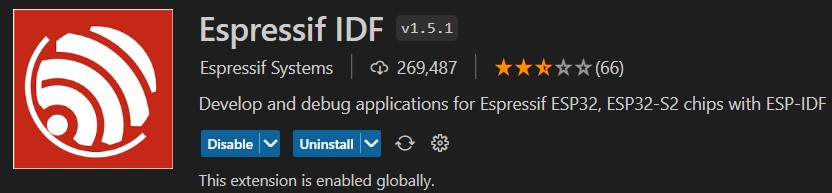
\includegraphics[width=12cm, height=6cm]{ListMaterialIDF}
		\caption{ESP-IDF Plug-In v1.5.1.} 
		\label{fig:ESP-IDF Plug-In v1.5.1.}
	\end{center}
\end{figure}
\end{itemize}

%%%%%%%%%%%%%%%%%%%%%%%%%%%%%%%
%\section{Software Bill Of Materials (SBOM)}

%%%%%%%%%%%%%%%%%%%%%%%%%%%%%%%

\section{Description of the Python Package: Keras}

For this project and in general for Machine Learning projects one of the most common packages required to ndertand for the development in python is Keras. In general, this is used to develop high-level neural networks, it is written in Python and is capable of running on top of TensorFlow. In the specific case of this project, Keras is been used in two stages, with the following tools: 
\begin{itemize}
	\item ImageDataGenerator, this tool provides a convenient and powerful way to load, pre-process, and augment image data for use in deep learning models. It allows to easy load image data from a directory structure, the application of pre-processing techniques, and the use of data augmentation to improve model performance.
	\item Layers, this tool is an essential component of a neural network model generation with Keras Package in python. A directed acyclic graph of the neural network is built using layers, where the output of one layer serves as the input for the following layer. Convolutional layers for image processing, recurrent layers for sequence data, and fully connected layers for dense neural networks are just a few of the pre-built layers available in the Keras framework. In the particular instance of this project, the following layers are mostly used for the implementation: 
	\begin{itemize}
		\item \textbf{Dense}, is also known as fully connected layer.  It links all the neurons from the layer below to the neurons in the layer above. A hyper-parameter that has to be determined is how many neurons are present in the dense layer. In this layer, the activation function can also be specified.
		\item \textbf{Conv2D}, is used for image processing. The input data is subjected to a convolution procedure, enabling the model to learn spatial hierarchies of features. The hyper-parameters of this layer may be categorized as the number of filters, kernel size, and strides.
		\item \textbf{MaxPool2D}, is used for down-sampling the input data. It decreases the spatial dimensions of the data by applying a max pooling operation to the input data. The hyper-parameters of this layer may be categorized as the pooling size and the strides.
		\item  \textbf{Flatten},  is used for flattening the multi-dimensional input data into a 1D array. It is frequently applied before the last dense layer in a model so that it can process the incoming data.
	\end{itemize}
\end{itemize}

Building a variety of neural network models for image classification and other image processing tasks, such object recognition and semantic segmentation, may be done by combining the Dense, Conv2D, MaxPool2D, and Flatten layers. To test out several designs and identify the one that best matches the data, the number and mix of these layers may be altered.

Keras' simplicity and ease of use are two of its key benefits. It abstracts away a significant portion of the complexity involved in creating and refining deep learning models, allowing developers to concentrate on the model's architecture and design rather than the specifics of its implementation.

Support for several back-ends, such as TensorFlow, Theano, and Microsoft Cognitive Toolkit, is another benefit of Keras (CNTK). As a result, programmers may create models and train them using any back end of their choosing, switching back-ends without having to alter the model's architecture or training code.

Also it is a simple package to install and use in Python, in order to do this, the following steps must be followed:
\begin{enumerate}
	\item Verify that Python is installed. This is done by running in the command prompt: \textls{python -V}.
	\item Install the required dependencies for Keras; numpy, scipy, and six. Run the following command in the command prompt: \textls{pip install numpy scipy six}.
	\item Install TensorFlow or one of the other supported backends. Keras is a high-level library that runs on top of TensorFlow, Theano, or Microsoft Cognitive Toolkit (CNTK). Run the following command: \textls{pip install tensorflow}.
	\item Install Keras by running the following command: \textls{pip install keras}.
\end{enumerate}

In order to test that Keras is properly installed, use this code: 
\begin{lstlisting}
	import keras; 
	print(keras.__version__)
\end{lstlisting}

As of now, the version of Keras being used is 2.9.0. Now lets present an example of how to use Keras in a simple python example:

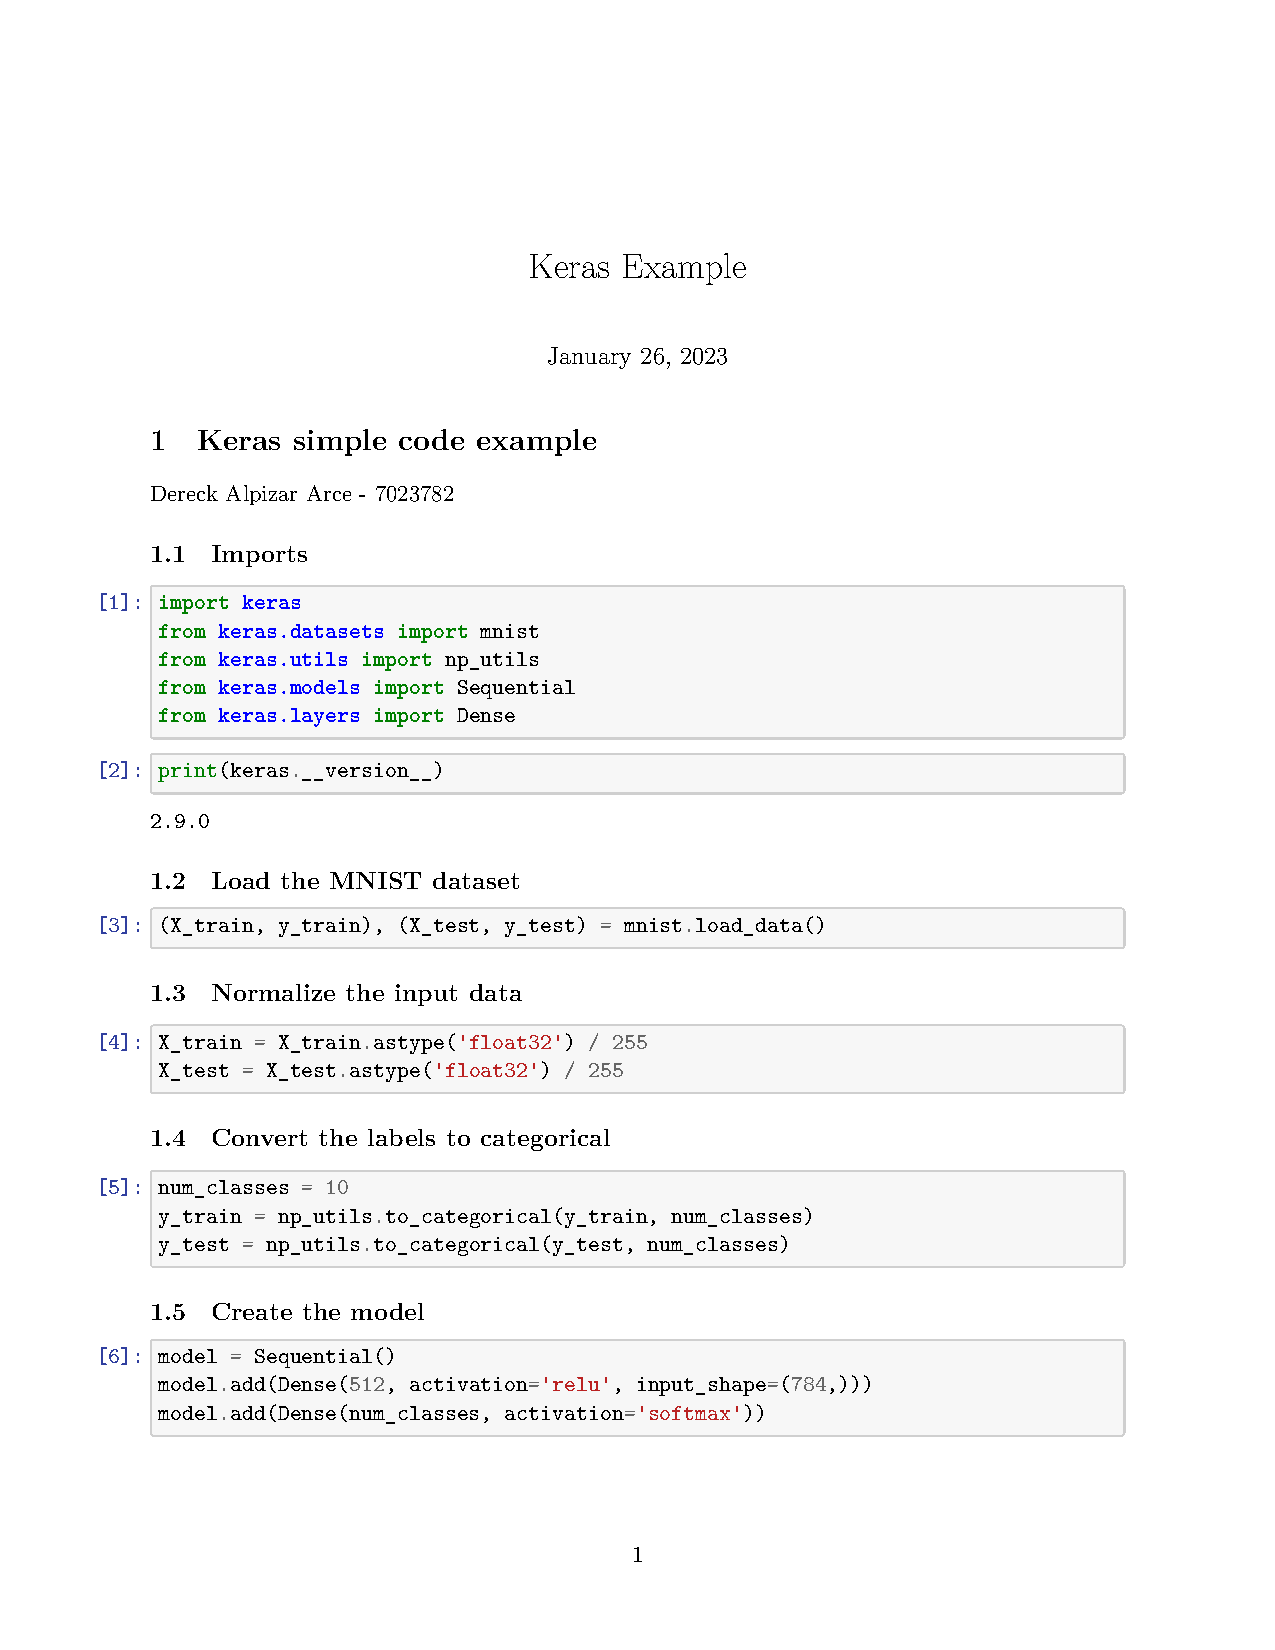
\includepdf[pages={-}]{Keras Example.pdf}

Lastly it is important to reference the developer source for Keras releases (past, current and next). In this GitHub repository one can access more detailed information regarding this package: \href[]{https://github.com/keras-team/keras/}{Keras: Deep Learning for humans}

%%%%%%%%%%%%%%%%%%%%%%%%%%%%%%%

\section{Description of the Python Package: NumPy}
Numerical Python (NumPy) is one of the most fundamental packages available in python for numerical computation. It is a general-purpose array-processing package which provides high-performance multidimensional arrays and appropriate tools to work with them. NumPy is capable of storing generic multi-dimensional data. In NumPy, dimensions are known as axes and the rank denotes the number of axes present. NumPy’s array class is termed as ndarray. \cite{Duggal:2022}\cite{Desai:2019} \\

\textbf{Functions:}

\begin{itemize}
	\item Computes basic array operations such as addition, multiplication, slicing, flatten, reshape and array indexing.
	\item Computes advanced array operations such as stacking arrays, splitting into sections and broadcasting arrays
	\item NumPy works with either Date Time or Linear Algebra
\end{itemize}

\textbf{Features:}

\begin{itemize}
	\item Provides pre-compiled functions for numerical routines 
	\item Array-oriented computing for better efficiency
	\item NumPy supports an object-oriented approach
	\item It is compact and performs faster computations with vectorization
\end{itemize}

\textbf{Applications:}

\begin{itemize}
	\item Predominantly used in data-analysis applications.
	\item Used for creating powerful N-dimensional array
	\item Forms the base of other libraries, such as SciPy and scikit-learn
	\item Used as a replacement of MATLAB when used with SciPy and matplotlib
\end{itemize}

\textbf{Installation}\\\\
To install Numpy, you can use the pip package manager by running the command "pip install numpy" in your terminal.\\

\textbf{Further Reading:}

\begin{itemize}
	\item The Numpy documentation (\url{https://numpy.org/doc/}) provides a comprehensive overview of the library's features and usage.
	\item The Scipy website (\url{https://scipy.org/}) also provides additional resources for scientific computing with Python, including tutorials and a user guide.
\end{itemize}
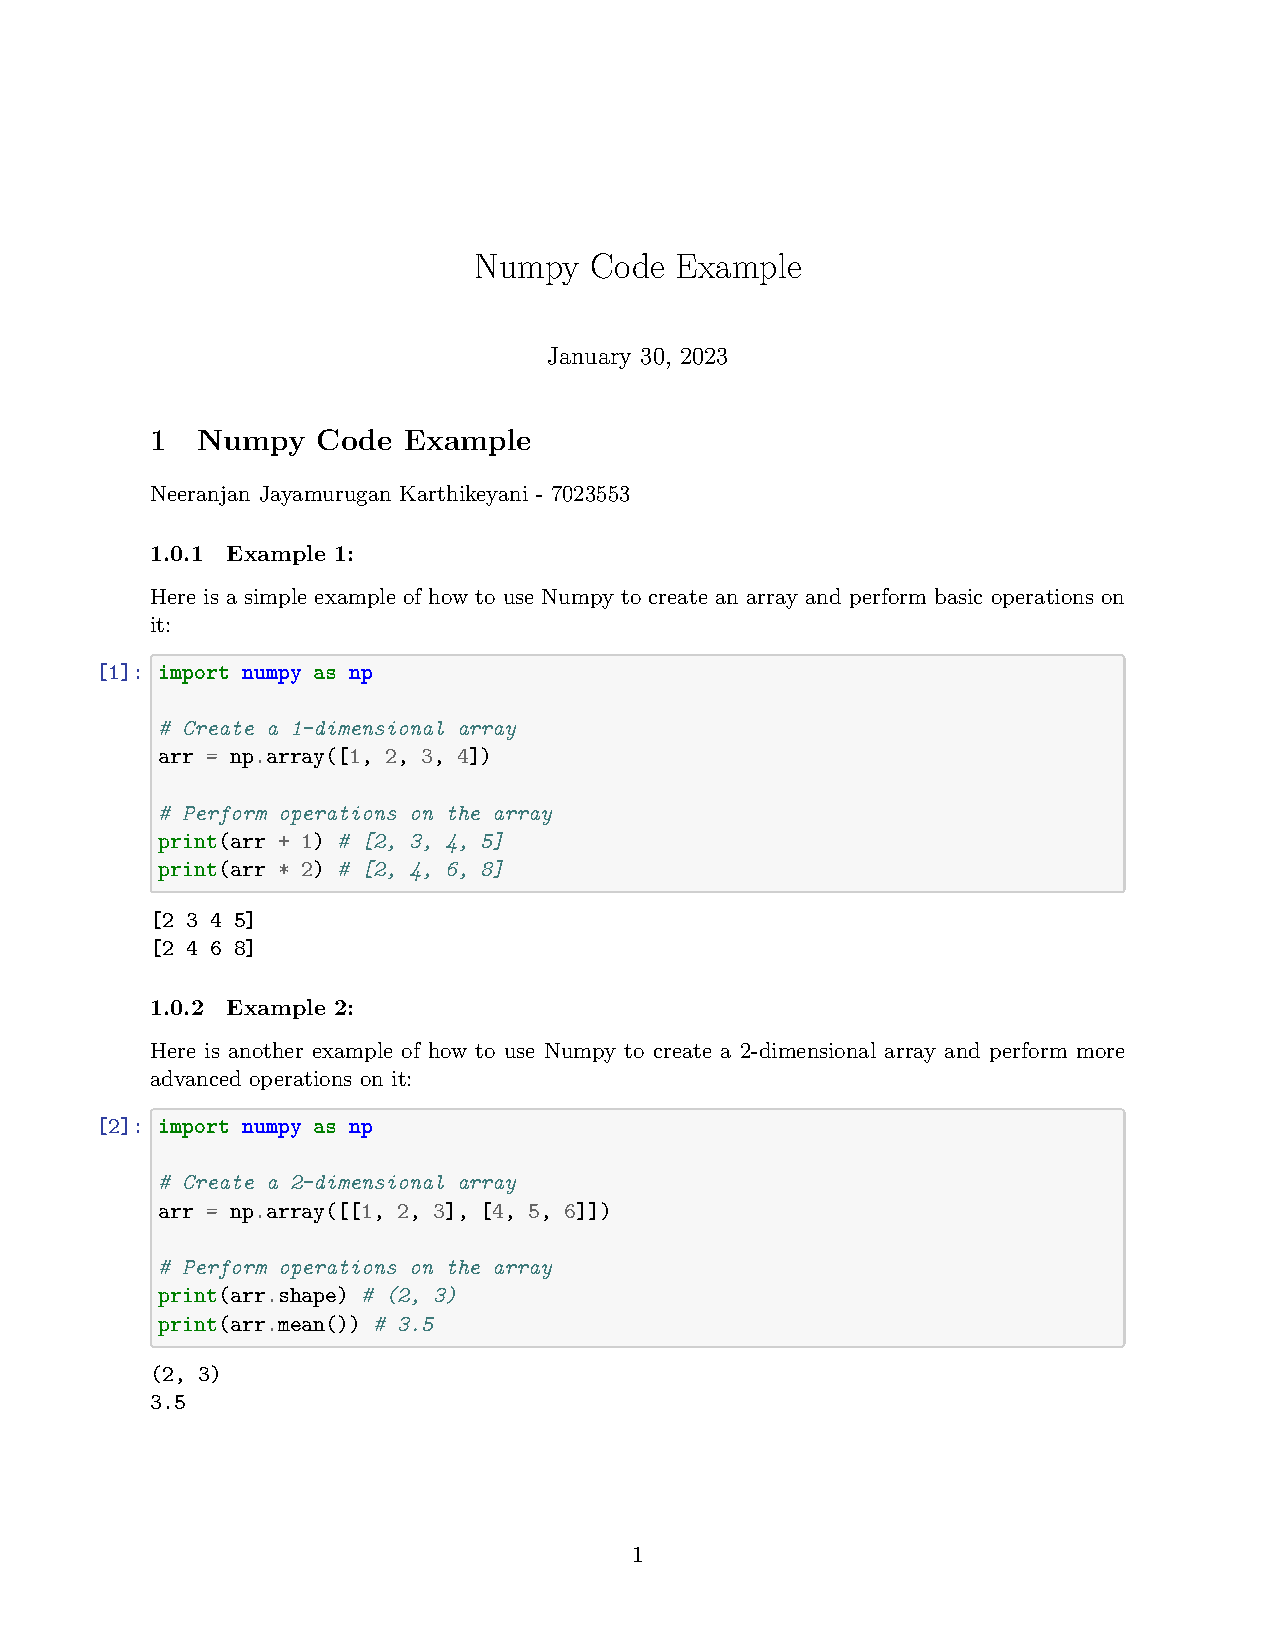
\includepdf[pages={-}]{NumpyCodeExample.pdf}

%%%%%%%%%%%%%%%%%%%%%%%%%%%%%%%

\section{Description of the Python Package: Matplotlib}

Matplotlib is an open-source drawing library which has powerful and wide range of visualizations. It extensively provides an object-oriented API which is used for embedding plots into applications. With the visualization capabilities of Matplotlib one can visualise everything that can be drawn from legends and grids to spectrogram. \cite{Duggal:2022}\cite{Desai:2019} \\

\textbf{Functions:}

With few lines of code, Matplotlib can depict a wide range of visualizations such as:
\begin{itemize}
	\item Line plots
	\item Scatter plots
	\item Area plots
	\item Bar charts and Histograms
	\item Pie charts
	\item Stem plots
	\item Contour plots
	\item Quiver plots
	\item Spectrograms
\end{itemize}

\textbf{Features:}

\begin{itemize}
	\item With the advantage of being open source, it can be used as a replacement for MATLAB.
	\item Supports dozens of backends and output types, which enables one to use it regardless of type of the operating system used or the output format used.
	\item Good runtime behavior and low memory consumption.
\end{itemize}

\textbf{Applications:}

\begin{itemize}
	\item Used for correlation analysis of variables.
	\item Used for visualizing 95 percent confidence intervals of the models.
	\item Outliers can be detected using a scatter plot.
	\item Can be used for visualizing the distribution of data to obtain instant insights.
\end{itemize}

\textbf{Installation}\\\\
Matplotlib can be installed using pip, conda, or by downloading the source code and running setup.py. It is recommended to install matplotlib through Anaconda distribution or using the command "pip install matplotlib".\\

\textbf{Further Reading:}

\begin{itemize}
	\item For more information on matplotlib, check out the official matplotlib documentation at \url{https://matplotlib.org/}.
\end{itemize}
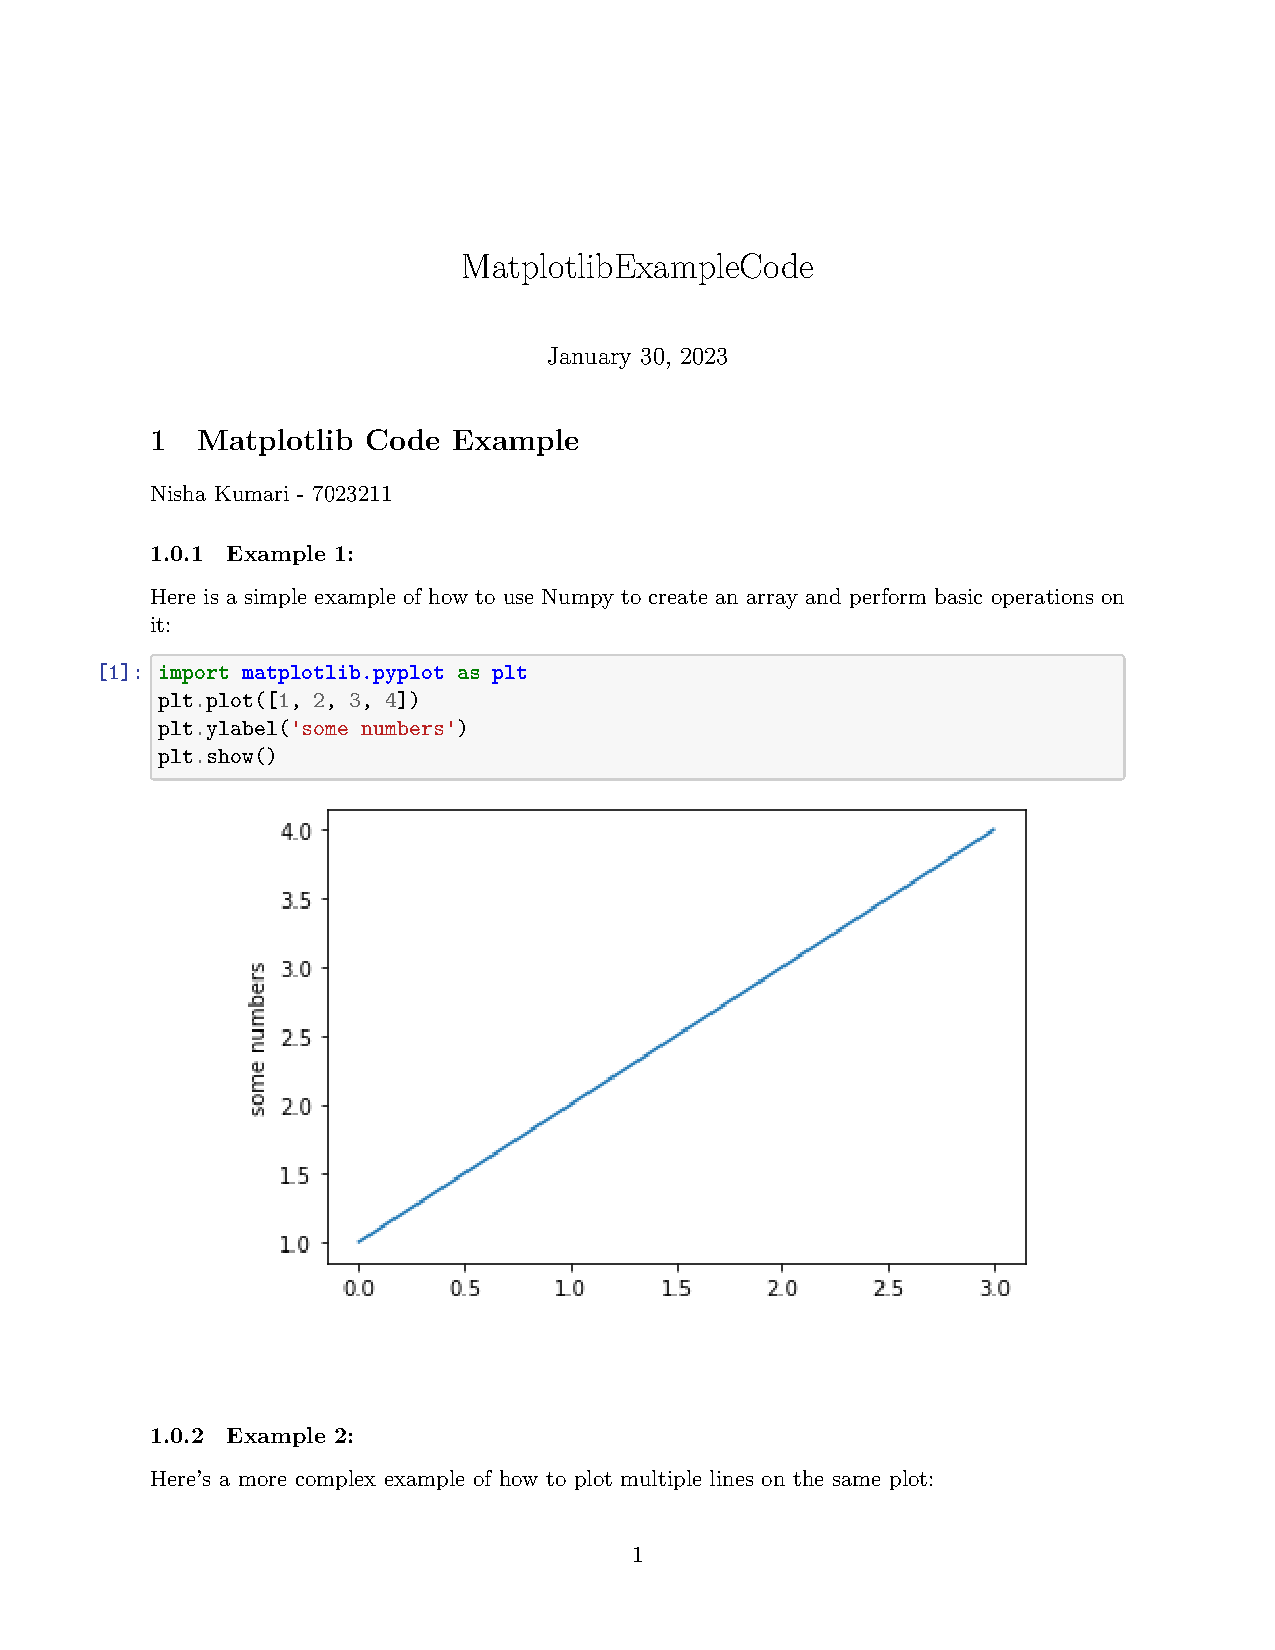
\includepdf[pages={-}]{MatplotlibExampleCode.pdf}

%%%%%%%%%%%%%%%%%%%%%%%%%%%%%%%